\documentclass[border=10pt]{standalone}
\usepackage{upgreek}
\usepackage[american]{circuitikz}
\usetikzlibrary{decorations.pathreplacing}
\usetikzlibrary{patterns}


\tikzset{
        hatch distance/.store in=\hatchdistance,
        hatch distance=3.5pt,
        hatch thickness/.store in=\hatchthickness,
        hatch thickness=0pt
    }
\makeatletter
\pgfdeclarepatternformonly[\hatchdistance,\hatchthickness]{flexible hatch}
    {\pgfqpoint{0pt}{0pt}}
    {\pgfqpoint{\hatchdistance}{\hatchdistance}}
    {\pgfpoint{\hatchdistance-1pt}{\hatchdistance-1pt}}%
    {
        \pgfsetcolor{\tikz@pattern@color}
        \pgfsetlinewidth{\hatchthickness}
        \pgfpathmoveto{\pgfqpoint{0.5pt}{0.5pt}}
        \pgfpathlineto{\pgfqpoint{\hatchdistance}{\hatchdistance}}
        \pgfusepath{stroke}
    }
\makeatother

\begin{document}
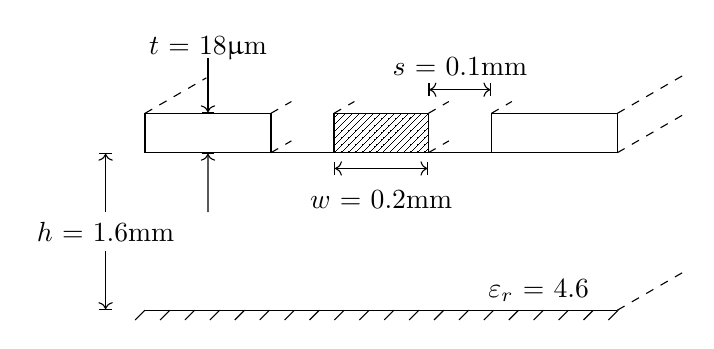
\begin{tikzpicture}
    % Use this to make edits
    % \draw[help lines, dashed] grid (6, 6);

    \draw (0,0) node[name=sw]{} -- ++ (6,0) node[name=se]{};
    \draw[
        draw = none,
        decoration = {border, segment length=9, amplitude=5, angle = -135},
        postaction = {decorate, draw}
    ] (0,0) -- ++ (6.5,0);
    \draw (0, 2) node[name=nw]{} -- ++ (6, 0) node[name=ne]{};
    \draw (6, 2)[dashed] -- ++ (30: 1);
    \draw (6, 0)[dashed] -- ++ (30: 1);
    % Trace (Width = 1.2)
    \draw[
        pattern = flexible hatch,
    ] (2.4, 2) node[name=ms-sw]{} rectangle (3.6, 2.5) node[name=ms-ne]{};
    \draw (3.6, 2)[dashed] -- ++ (30: 0.3);
    \draw (2.4, 2.5)[dashed] -- ++ (30: 0.3);
    \draw (3.6, 2.5)[dashed] -- ++ (30: 0.3);
    % Coplanar GND (Width = 2.6)
    \draw (0, 2) rectangle ++ (1.6, 0.5);
    \draw (4.4, 2) rectangle ++ (1.6, 0.5);
    \draw (0, 2.5)[dashed] -- ++ (30: 0.9);
    \draw (6, 2.5)[dashed] -- ++ (30: 1);
    \draw (1.6, 2)[dashed] -- ++ (30: 0.3);
    \draw (1.6, 2.5)[dashed] -- ++ (30: 0.3);
    \draw (4.4, 2.5)[dashed] -- ++ (30: 0.3);
    % Gap (Width = 0.8)
    \draw (3.6, 2.8)[|<->|] -- (4.4, 2.8);
    \draw (4, 3.1) node{$s$ = 0.1mm};
    % Height
    \draw (-0.5, 1) node[name = height]{$h$ = 1.6mm};
    \draw (height.north)[->|] -- (-0.5,2);
    \draw (height.south)[->|] -- (-0.5,0);
    % Width
    \draw (2.4, 1.8)[|<->|] -- (3.6, 1.8);
    \draw (3, 1.4) node{$w$ = 0.2mm};
    % Thickness
    \draw (height.north) ++ (1.3, 0)[->|] -- (0.8, 2);
    \draw (0.8, 2.5)[|<-] -- ++ (0, 0.7) node[name=t]{};
    \draw (t.north) node{$t$ = 18$\upmu$m};
    % Dielectric Constant
    \draw (5, 0.25) node[name = er]{$\varepsilon_r$ = 4.6};
\end{tikzpicture}
\end{document}